%! Author = David Nabergoj
%! Date = 31/01/2021

% Preamble
\documentclass[11pt, twocolumn]{article}

% Packages
\usepackage{graphicx}
\usepackage{amsmath}
\usepackage{amsfonts}
\usepackage[htt]{hyphenat}
\usepackage[
    top=19mm,
    bottom=19mm,
    left=19mm,
    right=19mm
]{geometry}
\usepackage{hyperref}
\hypersetup{
    colorlinks=true,
    linkcolor=red,
    urlcolor=blue,
    citecolor=black
}
\urlstyle{same}

%\newenvironment{disclaimer}
%    {
%    \begin{center}
%    \begin{tabular}{|p{0.9\hsize}|}
%    \hline\\
%    \begin{footnotesize}\textbf{Disclaimer.}}
%    {
%    \end{footnotesize}
%    \\\\\hline
%    \end{tabular}
%    \end{center}
%    }

% Title, author
\title{Reproducibility report: Walsh-Hadamard Variational Inference for Bayesian Deep Learning}
\author{David Nabergoj\thanks{University of Ljubljana, david.nabergoj@student.uni-lj.si}}

% Document
\begin{document}
    \maketitle

    \section{Introduction}\label{sec:introduction}
    In this report, we assess the reproducibility of the paper ``Walsh-Hadamard Variational Inference for Bayesian Deep Learning''~\cite{rossi2019walsh}.
Our results are based on multiple readings of the original paper and its supplementary material, re-runs of the described experiments, as well as some key referenced literature~\cite{le2014fastfood, blundell2015weight, fino1976unified, kingma2015variational, rossi2019good}.
This reproduction is not based on any published code, except the CUDA implementation of the fast Walsh Hadamard transform by the paper's authors.
Our implementation of the proposed method, experiments and other related files are available at \url{https://github.com/davidnabergoj/WHVI}.

\subsection{Brief review of the paper}\label{subsec:brief-review-of-the-paper}
The authors propose Walsh-Hadamard Variational Inference (WHVI), where weight matrices in Bayesian neural networks are efficiently re-parameterized to allow for linear space complexity and log-linear time complexity when transforming an input vector with a WHVI layer.
The key idea is that weight matrices can be efficiently sampled by
\begin{align}
    \widetilde{\mathbf{W}} = \mathbf{S_1} \mathbf{H} \mathrm{diag}(\widetilde{\mathbf{g}}) \mathbf{H} \mathbf{S_2},\quad\widetilde{\mathbf{g}} \sim q(\mathbf{g}).
    \label{eqn:weight-sampling}
\end{align}
Here, $\widetilde{\mathbf{W}}$ is a $D \times D$ weight matrix sample, $\mathbf{S_1}$ and $\mathbf{S_2}$ are deterministic diagonal matrices whose entries need to be optimized, $\mathbf{H}$ is the Walsh-Hadamard matrix, and $\widetilde{\mathbf{g}}$ is a sample from the distribution $q$.
The variational posterior distribution $q$ is a multivariate normal distribution with a diagonal covariance matrix, i.e.\ $q(\mathbf{g}) = \mathcal{N}(\mathbf{\mu}, \mathbf{\Sigma})$.

This approach offers an advantage over other approaches like Mean field Gaussian variational inference, because it requires $O(D)$ instead of $O(D^2)$ parameters to represent weight matrices of size $D \times D$.
Furthermore, the matrix-vector product $\mathbf{Hx}$ can be computed in $O(D \log D)$ time and $O(1)$ space using the in-place version of the Fast Walsh-Hadamard transform.
The reduced number of parameters causes the KL term to be less dominant during model training, which is otherwise a common problem in Bayesian deep learning.
The described approach supports matrices of size $D \times D$ where $D = 2^p$ for $p > 0$ in its most basic form, however it is extended to support matrices of arbitrary size by concatenating smaller square matrices.

WHVI is applied to a toy example, several regression data sets, and is also tested on image classification tasks using Bayesian convolutional neural networks.

\subsection{Reproducibility goals}\label{subsec:reproducibility-goals}
Our main goal is to implement all required procedures for WHVI and run the described experiments.

We first try to reproduce results for the toy univariate regression example in section 3.1 of the original report.
This primarily means obtaining qualitatively similar uncertainty estimates.
We then focus on the regression data sets, as listed in Table 3 of the original report.
The goal is to obtain similar WHVI test error and WHVI test MNLL (mean negative log-likelihood) estimates, both the mean and the standard deviation.

Due to long training times for Bayesian neural networks, complex convolutional neural network architectures, and the large number of parameters ($\sim 2.3$M), we do not consider image classification experiments in this report.
We believe they are not crucial to assessing the quality of the proposed approach, because linear layers (not involving convolution operations) are already evaluated using standard regression data sets, whereas the authors report that using WHVI for convolutional filters does not yield interesting results due to the small number of parameters.
We focus only on mean-field WHVI and not on the version involving normalizing flows, which are mentioned as an extension to the proposed method.

We attempt to reproduce the findings regarding WHVI inference time to a smaller degree, because the workstation used in the experiments of the original paper is significantly more powerful than the one we used in this reproduction study.
We compare the speed of matrix multiplication and fast Walsh-Hadamard transform on the CPU and the GPU, but not the experiments regarding energy consumption.
We test the method across different random seeds to empirically assess stability and convergence.

\subsection{Report structure}\label{subsec:report-structure}
We describe our implementation of the proposed method in Section~\ref{sec:implementation-details}.  % TODO say more
We compare our results to those in the original paper in Section~\ref{sec:model-testing}, where we discuss the inference process, predictive quality, and compute performance.
In Section~\ref{sec:conclusion-and-discussion}, we conclude the report with an overall reproducibility assessment provide some suggestions for improvement.


    \section{Implementation details}\label{sec:implementation-details}
    In this section, we describe our implementation of WHVI and list assumptions for parts which were not described in detail in the original paper.
We discuss the core classes, FWHT, setting the prior, and initializations for parameters.
\subsection{Core classes}\label{subsec:core-classes}
We implemented WHVI in PyTorch~\cite{pytorch}, because it is also used in the original paper.
The most important part is the \texttt{WHVISquarePow2Matrix} class, which contains as parameters the elements of $\mathbf{S}_1$, $\mathbf{S}_2$, and the posterior mean $\mu$.

The authors do not state how they represent $\Sigma$.
We do not directly use the elements of the diagonal covariance matrix $\Sigma$, but instead use a parameter vector $\rho$ with $D$ elements, which corresponds to $\Sigma$ via a softplus transformation: $\Sigma = \mathrm{diag}(\sigma_1, \dots, \sigma_D)$ where $\sigma_i = \ln(1 + \exp(\rho_i))$.
We choose the softplus transformation, because it was used in the seminal work on variational inference in neural networks~\cite{blundell2015weight}.
The advantage is that we can optimize $\rho_i$ across the real line and disregard positivity constraints in the gradient-based optimization, then ensure non-negativity via a simple transformation.
We acknowledge that the referenced work uses softplus for individual elements of the weight matrix, whereas we use it for elements of vector $\mathbf{g}$, which is indirectly related to the weight matrix via Equation~\ref{eqn:weight-sampling}.

To transform a batch of input vectors, a weight matrix is sampled from the posterior according to Equation~\ref{eqn:weight-sampling} and multiplied by a matrix whose rows are vectors from that batch.
We implemented two options for this transformation.
In the first, we sample the weight matrix directly according to Equation~\ref{eqn:weight-sampling}.
In the second, we use the local re-parameterization trick to sample the matrix-vector product $\mathbf{W}\mathbf{x} \in \mathbb{R}^D$ according to Equations~\ref{eqn:lrt1} and~\ref{eqn:lrt2}.
\begin{align}
    \mathbf{W}\mathbf{x} = \overline{\mathbf{W}}(\mathbf{\mu})\mathbf{x} + \overline{\mathbf{W}}(\mathbf{\Sigma}^{1/2}\mathbf{\epsilon})\mathbf{x}, \; \epsilon \sim \mathrm{N}(\mathbf{0}, \mathbf{I}_D)\label{eqn:lrt1},\\
    \overline{\mathbf{W}}(u) = \mathbf{S}_1 \mathbf{H} \mathrm{diag}(\mathbf{u}) \mathbf{H} \mathbf{S}_2\label{eqn:lrt2}
\end{align}
We use the second option as it is not too slow when compared to the first, but has the advantage of decreasing the variance of stochastic gradients.
For example, the number of epochs per second decreases from 190 to 155 on the toy dataset from Section 3.1 of the original paper.

The \texttt{WHVIStackedMatrix} class represents matrices of arbitrary size.
It identifies how many smaller matrices of type \texttt{WHVISquarePow2Matrix} need to be stacked together to allow for the desired matrix multiplication, as well as the necessary padding of the input vector (see Algorithm 1 in the original report).
These smaller matrices are stored in a \texttt{ModuleList} container as an attribute of \texttt{WHVIStackedMatrix}.
When transforming a batch of input vectors, we generate one sample for each small matrix and concatenate these samples into a large matrix.
The inputs are padded as necessary.

As a special case, we also implement the \texttt{WHVIColumnMatrix} class, which transforms a batch of input vectors with a single element into a batch of output vectors with many elements.
It includes a smaller \texttt{WHVISquarePow2Matrix}, which is sampled at input transformation time and reshaped into a column.
The last few elements of this column may be removed to accommodate for the desired output size.
This method is recommended in the paper and indeed reduces the number of parameters from $O(D)$ to $O(\sqrt{D})$, while also reducing the single-vector transform time complexity from $O(D\log D)$ to $O(\sqrt{D}\log D)$.
Note that by transposing the sampled matrix, this class can be used to map many inputs to a single output.

Finally, we create a \texttt{WHVILinear} layer class, which automatically selects the appropriate matrix based on the desired input and output dimensionalities.
This is analogous to the traditional \texttt{Linear} layer in PyTorch, but also includes the computation of KL divergence $D_\mathrm{KL}\left(q(\mathbf{g}|\mu, \Sigma)\, ||\, p(\mathbf{g})\right)$ from the prior $p$ to the variational posterior $q$.
The KL divergence of a \texttt{WHVILinear} layer is the sum of KL divergence terms for all of its descendants of type \texttt{WHVIStackedMatrix}.

\subsection{Fast Walsh-Hadamard transform}\label{subsec:fast-walsh-hadamard-transform}
An important contribution of the paper is the use of FWHT~\cite{fino1976unified}, which allows for log-linear vector transformation time.
We implemented the transform in Python and C++, both implementations can be used on the CPU and the GPU\@.
We also adapted and tested a CUDA kernel implementation, which is considerably faster than the Python and C++ implementations on the GPU\@.
The performance is described more thoroughly in Section~\ref{fig:compute-performance} with additional comparisons to regular matrix multiplication.

\subsection{Priors and parameter initializations}\label{subsec:priors-and-parameter-initializations}
According to the supplementary material for the original paper, we use a zero-mean prior with fully factorized covariance $\lambda \mathbf{I}$ for a particular layer, i.e. $\mathcal{N}(\mathbf{0}, \mathrm{diag}(\lambda, \dots, \lambda)$ for a chosen $\lambda > 0$.

We believe that the original paper should describe the choices of prior variances in more detail.
Currently, the supplement seems to suggest that a constant $\lambda = 10^{-5}$ was used in all layers of the deep Bayesian networks, but this is likely not the case.
By reconsidering the statement in the supplement, we may interpret it as putting a low prior covariance on the last layer and possibly higher ones on the previous layers.
Good choices of $\lambda$ are thus essential at each layer separately.

The authors did not describe the initialization of $\mathbf{S}_1$, $\mathbf{S}_2$, $\Sigma$.
We draw initial elements of $\mathbf{S}_1$ and $\mathbf{S}_2$ i.i.d.\ from $\mathrm{N}(0, 0.01)$ and initial elements of $\rho$ i.i.d.\ from Uniform$(-3, -2)$.


    \section{Model testing}\label{sec:model-testing}
    In this section, we test our WHVI implementation, specifically the inference and predictive quality of Bayesian deep neural networks that use WHVI linear layers.
We first focus on the toy example from Section 3.1 and then discuss regression experiments from Section 3.2 of the original paper.
% Some discrepancies on the toy example are already large enough that more complex experimentation is not meaningful.

\subsection{Toy example}\label{subsec:toy-example}
We consider the toy example from Section 3.1 in the original paper.
The authors do not provide an explicit formula for the function.
To replicate the experiment as closely as possible, we look at the plot and roughly observe some $(x, y)$ pairs -- extrema and in-between values.
We then use polynomial interpolation with a Vandermonde matrix to obtain a similar-looking function.
This function is visualized in Figure~\ref{fig:toy-function}.

\begin{figure}[h]
    \centering
    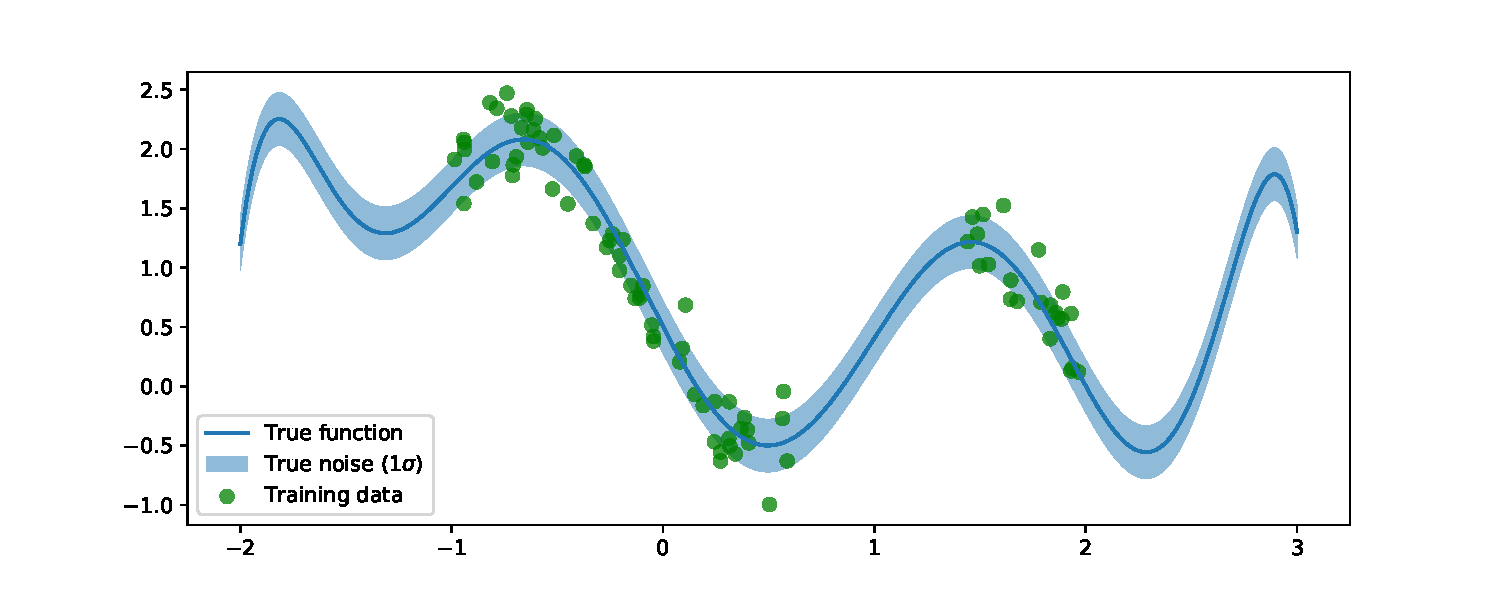
\includegraphics[width=1.0\hsize]{img/toy-function}
    \caption{Polynomial approximation to the toy function in the original paper.
    The exact form of this function up to two decimals is $f(x) = 0.50 -3.45x + 1.14x^2 + 4.36x^3 -0.93x^4 -1.77x^5 + 0.39x^6 + 0.22x^7 -0.06x^8$.
    The noise is normally distributed with $\sigma = \sqrt{\exp (-3)}$.
    }
    \label{fig:toy-function}
\end{figure}

The cosine activation function is no longer suitable given this different form of the function.
We check this by training a non-Bayesian model, which has the exact same architecture as the WHVI one (two hidden layers with 128 hidden units).
We found that the sigmoid activation performs slightly better and decided to use it in the WHVI experiment instead.
A comparison of the two non-Bayesian models with different activations can be seen in Figure~\ref{fig:toy-function-non-bayesian}.

\begin{figure}
    \centering
    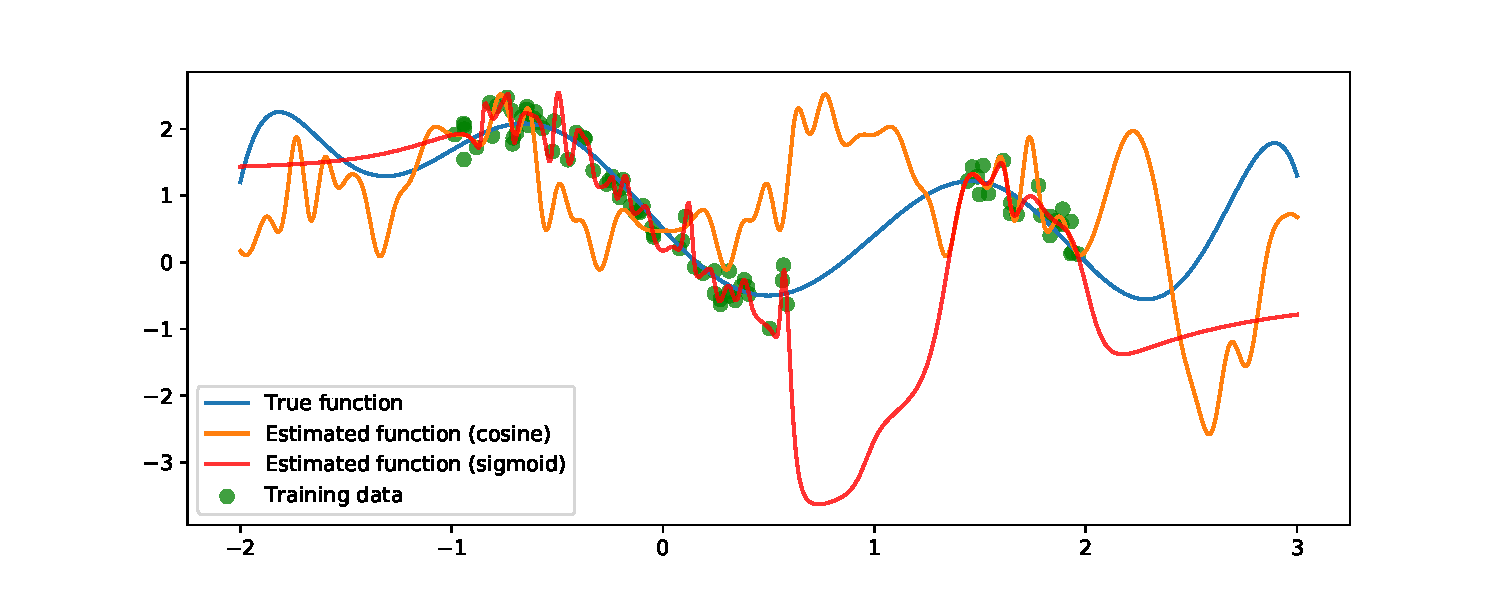
\includegraphics[width=1.0\hsize]{img/toy-function-non-bayesian}
    \caption{Comparison of the cosine and the sigmoid activation in a non-bayesian network.
    We decided to use sigmoid instead of cosine, because it seemed to capture the function more nicely on the left chunk of the data.}
    \label{fig:toy-function-non-bayesian}
\end{figure}

We trained the model with WHVI layers and found that the results depend heavily on initial $\lambda$ values in each layer as well as the initial scale $\sigma_0$ of the Gaussian likelihood.
The result is visualized in Figure~\ref{fig:toy-function-whvi}.
\begin{figure}[htbp]
    \centering
    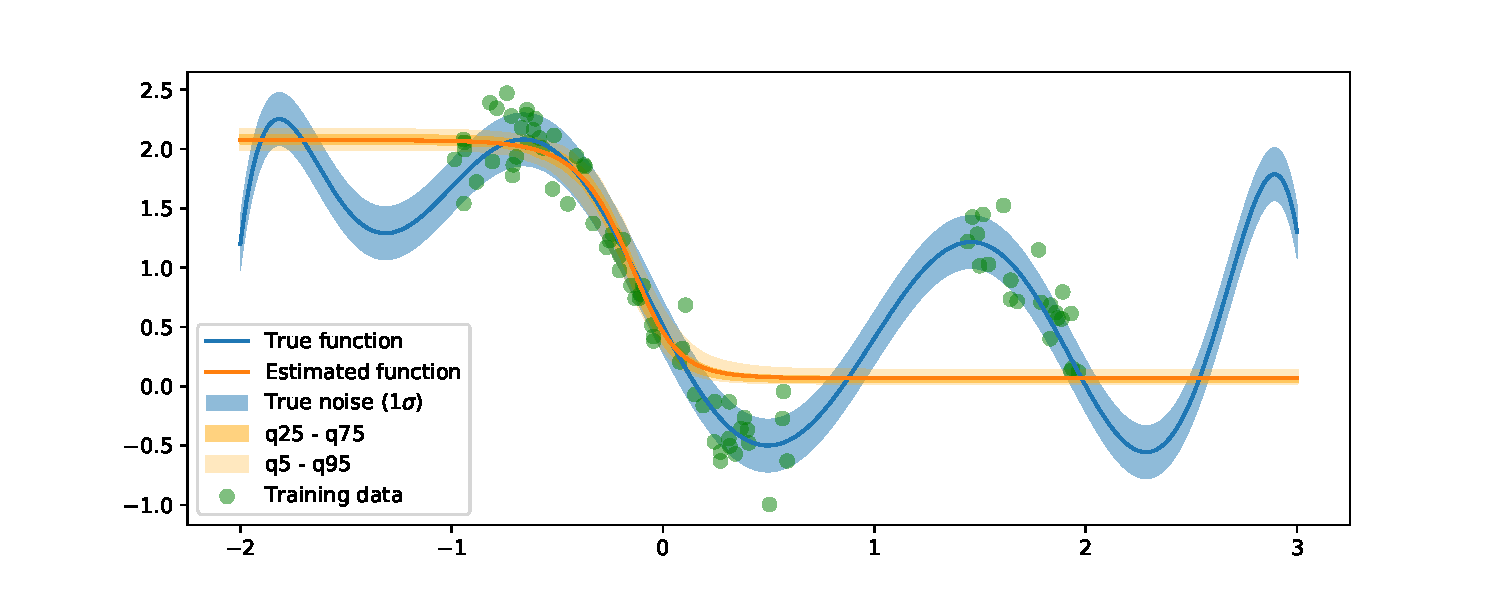
\includegraphics[width=1.0\hsize]{img/bayesian-fit-with-kl}
    \caption{
    Estimated function and the corresponding uncertainty.
    The dark-shaded region represents quantiles $q_{25}-q_{75}$, whereas the bright-shaded one represents $q_{5}-q_{95}$.
    The underlying function is not modeled well.
    The model remains stuck in this local minimum even if we increase the number of epochs from 50000 to 200000.}
    \label{fig:toy-function-whvi}
\end{figure}

Many parameter choices resulted in slow convergence and significantly underestimated uncertainty.
Our suggestions are to set $\lambda$ values that get gradually smaller as we approach the output layer and set $\sigma_0$ to be sufficiently larger than zero.
In particular, our choices for modeling the toy data set were $\lambda_1=15, \lambda_2=15,\lambda_3=0.01, \sigma_0=5$.
We also observed that the KL term in ELBO would often be much larger than the MNLL term at the beginning of the optimization.
Conversely, the MNLL term would get stuck at suboptimal value and be unable to escape this local minimum even after several thousand epochs.
After optimization, we observed several times that all but one pair of $\mu$ and $\Sigma$ parameters were almost exactly equal to zero and $\lambda$, indicating that the KL term was too dominant, drawing the variational posterior too close to the prior.

The authors also state that they obtained a model with 1541 parameters for the toy example, however we obtained one with 1537 parameters.
We were not able to identify the missing parameters and we believe that they are not hyperparameters, because the authors refer to hyperparameters separately in a Supplement section (i.e.\ not as ``parameters'').
These missing parameters might be the solution to the observed problems in our experiments.

As an attempt to improve performance, we added bias columns (to be optimized) to WHVI layers.
This addition was not enough to obtain the desired results and also introduced a considerably large number of additional parameters.
We suggest further research regarding parameter initialization.
A possible solution would be to explore hyperpriors for $\mu$ and $\rho$ to allow for greater flexibility in the sampled weights.
We found the choice of random seed not to improve results by observing the fit with seeds $5000k, k = \{1, \dots, 10\}$.
To conclude, we were not able to reproduce the uncertainty estimates, presented in the original paper.

\subsection{Regression experiments}\label{subsec:regression-experiments}
This section refers to experiments in section 3.2 and Table 3 of the original paper.
We use the experimental setup as described in section 3.2 of the original paper and section D.1 of the Supplement.
Again, the paper does not state the prior covariances $\lambda$ except for the last layer, where $\lambda = 10^{-5}$.
We choose $\lambda = 3$ for all previous layers.

The comparison between our results and the ones from the paper are presented in Table~\ref{tab:regression-experiments}.
\begin{table*}[]
    \begin{tabular}{l|llll}
               & RMSE (original) & RMSE (ours) & { }MNLL (original) & MNLL (ours) \\ \hline
    Boston     & 3.14 (0.71)     &             & { }4.33 (1.80)     &             \\
    Concrete   & 4.70 (0.72)     &             & { }3.17 (0.37)     &             \\
    Energy     & 0.58 (0.07)     &             & { }2.00 (0.60)     &             \\
    KIN8NM     & 0.08 (0.00)     &             & -1.19 (0.04)       &             \\
    Naval      & 0.01 (0.00)     &             & -6.25 (0.01)       &             \\
    Powerplant & 4.00 (0.12)     &             & { }2.71 (0.03)     &             \\
    Protein    & 4.36 (0.11)     &             & { }2.79 (0.01)     &             \\
    Yacht      & 0.69 (0.16)     &             & { }1.80 (1.01)     &
    \end{tabular}
    \caption{WHVI regression experiments results. RMSE and MNLL are computed on test data sets. The result format is \textit{mean (std)}, where the sample mean and standard deviation are computed across 8 independent random train-test splits of the data sets.}
    \label{tab:regression-experiments}
\end{table*}
We were unable to reproduce the results, shown in the original paper.
We believe that this is due to the missing parameters (see Subsection~\ref{subsec:toy-example}) and possibly due to different values of $\lambda$.
It is also possible that the authors invested more time into hyperparameter tuning to achieve such results, however we were unable to do the same given the considerable time and computational resources required for the experiments.

We do not evaluate WHVI performance further, because it is clear that the lack of parameters and/or the choice prior initializations are causing poor results.


    \section{Performance testing}\label{sec:performance-testing}
    % Present results
% Explain results

In this section, we discuss the computational efficiency of our implementation of WHVI and FWHT\@.

% It is not clear from the original paper to what extent the in-place version of FWHT was utilized.
% We found that using in-place operations caused problems in the PyTorch autodifferentiation engine so that the computed gradient was incorrect.
% We consequently cloned the input batch before using the transform, but this did not noticeably decrease processing speed.

The CUDA implementation of FWHT was not explained in the original paper or the supplement.
We adapted an implementation of the kernel from the original paper\footnote{See the author's repository at \url{https://github.com/srossi93/vardl} and a somewhat different implementation of the transform at \url{https://github.com/HazyResearch/structured-nets}.} and used it in our experiments.
We suggest reading the paper by Bikov and Bouyukliev (2018)~\cite{bikov2018parallel} for a clear and concise FWHT implementation reference, as well as the detailed implementation strategies, described by Arndt (2010)~\cite{arndt2010matters}.


    \section{Conclusion and discussion}\label{sec:conclusion-and-discussion}
    We implemented Walsh-Hadamard Variational Inference as proposed in the original paper.
The main contribution of the method is the significantly reduced number of parameters needed to represent a weight matrix in a Bayesian neural network and the use of the fast Walsh-Hadamard transform for time and space-efficient computations.

We were not able to reproduce the findings in the original paper with our implementation.
We believe that this is primarily because of missing parameters, which we were unable to identify.
Another possibility is the choice of hyperparameters, parameter initialization strategies, and prior selection, which could have been discussed somewhat more in the original paper.
We realize that some of these details and other common knowledge in variational inference might have been omitted from the published paper and the supplement due to space constraints.
Over the course of this reproduction, we were able to find some answers to our questions in the cited papers.

We contacted the authors regarding the issues, and they were kind enough to link the Github repository\footnote{\url{https://github.com/srossi93/vardl}} with some supporting code for the paper.
We would like to express our gratitude for this help.
While the linked repository contains code for some methods, it is still in development and yet to be thoroughly documented.
Unfortunately, the notebooks for the studied paper are also not available.
Due to time constraints, we cannot study the code in detail at the time of writing.
However, after checking some related classes, we saw some procedures that were not described in the paper.
For example, there is support for biases in the WHVI layers, but because there are no notebooks, it is unclear which of the experiments used biases and which did not.
We will update our code and this report once the authors publish additional materials for the paper.


    \bibliographystyle{unsrt}
    \bibliography{bibliography}

\end{document}